\documentclass[11pt]{article}

\usepackage{amsmath}
\usepackage{amsfonts} 
\usepackage{amsthm}
\usepackage{blkarray}
\usepackage{caption}
\usepackage{enumitem} 
\usepackage{mathtools}
\usepackage{tikz}
\usepackage[top=2cm,bottom=2cm,left=2cm,right=2cm,marginparwidth=1.75cm]{geometry}
\setlength{\parindent}{0cm}

\newcommand{\R}{\mathbb{R}}
\newcommand\simpleGraph[1]{
  \begin{tikzpicture}[every node/.style={circle,draw}]
    \node (a) at (0,1) {};
    \node (b) at (1,1) {};
    \node (c) at (1,0) {};
    \node (d) at (0,0) {};

    \foreach \from/\to in {#1}
      \draw (\from) -- (\to);
  \end{tikzpicture}\hfil
}
\newcommand\itm[1]{\item[\textbf{#1}]}
\newcommand{\incid}{{-}\!{\bullet}\!{-}}
\newcommand{\n}{\vspace{0.5cm}}

\def\lc{\left\lceil}   
\def\rc{\right\rceil}
\def\lf{\left\lfloor}   
\def\rf{\right\rfloor}

\newtheorem{theorem}{Theorem}

\title{\vspace{-1.0cm}MATH 5707 Midterm 1}
\author{Fletcher Gornick}
\date{February 25, 2022}

\begin{document}
\maketitle
  \begin{enumerate}
    \item (20 points) \textbf{True} or \textbf{False}.  To receive full credit, assertions which are true must be proven, and those that are false must have a counterexample exhibited.
      \begin{enumerate}
        \item (5 points) There exists a \textbf{simple} graph (no loops, no parallel edges) having degree sequence \((d_1, \hdots, d_n) = (6,6,6,6,5,3,3,1)\). \n\\
          \textbf{FALSE}.  In homework 1, the Havel-Hakimi algorithm was proven.  It states that, given graph \(G = (V,E)\) with corresponding (non-decreasing) degree sequence \((d_1, \hdots, d_n)\), \(G\) is graphic if and only if the graph corresponding to degree sequence \((d_2-1, \hdots, d_{d_1+1}-1, d_{d_1+2}, \hdots, d_n)\) is.
          \begin{align*}
            (6,6,6,6,5,3,3,1) &\to (5,5,5,4,2,2,1) \\
                              &\to (4,4,3,1,1,1) \\
                              &\to (3,2,0,0,1) \\
                              &\to (3,2,1)
          \end{align*}
          In this last degree sequence, we have 3 vertices, one of which has degree 3.  This means that there must either be a loop or a double link, thus \(G\) cannot be a simple graph. \n

        \item (5 points) For \(a,b \geq 1\), the complete bipartite graph \(K_{a,b}\) is eulerian if and only if \(a,b\) are both even. \n\\
          \textbf{TRUE}.  By theorem 4.1, a graph is eulerian if and only if it has no vertices with odd degree.  So, without loss of generality,  if \(a\) was odd, then all \(b\) vertices in one side of our complete bipartite graph would have degree \(a\) which is odd making \(K_{a,b}\) not eulerian by theorem 4.1. \n\\
          If \(a\) and \(b\) are both even, then we can conclude that every vertex in \(K_{a,b}\) has even degree and thus, must be eulerian. \n

        \item (5 points) For \(a,b \geq 2\), the complete bipartite graph \(K_{a,b}\) is hamiltonian if and only if \(a = b\). \n\\
          \textbf{FALSE}.  While it is necessary that \(a = b\) for \(K_{a,b}\) to be hamiltonian, it's not always sufficient.  Take \(K_{1,1}\) for example.  There exists a Hamilton path, just take the only edge in the graph, but there is no cycle, so \(K_{1,1}\) cannot be hamiltonian. \n

        \item (5 points) Any simple graph contains either an Euler tour or Hamilton cycle, or both. \n\\
          \textbf{FALSE}.  Take any disconnected set as a counterexample.  You could even take any tree.  Any simple graph without a cycle cannot contain an Euler tour or a Hamilton cycle either.
      \end{enumerate}

      \newpage
    \item (20 points) Given a multigraph \(G = (V,E)\) and any edge-cost function \(c \colon E \to \R_{\geq 0}\), let \(T\) be a minimum cost spanning tree, that is, a spanning tree \(T \subseteq E\) that achieves the smallest value of 
      \[c(T) := \sum_{e \in T} c(e).\]
      \textbf{Prove or disprove (via counterexample)}: For every pair of vertices \(x,y \in V\), the unique path \(P\) from \(x\) to \(y\) within \(T\) will achieve the minimum cost \(c(P)\) among \textit{all} paths from \(x\) to \(y\) within \(G\). \n\\
      This is false.
      \begin{proof}
        Take, for example, the following graph:

        \begin{minipage}{0.4\textwidth}
          \centering
            \begin{tikzpicture}
              \node(v1) at (0.5,0) {\(z\)};
              \node(v2) at (2,2) {\(x\)};
              \node(v3) at (3.5,0) {\(y\)};

              \node(c1) at (1.25,1) {\(5\)};
              \node(c2) at (2.75,1) {\(8\)};
              \node(c3) at (2,0) {\(6\)};

              \filldraw[black] (0,1) circle (0pt) node[anchor=center]{\(G = \)};
              \draw (v1) -- (c1) -- (v2) -- (c2) -- (v3) -- (c3) -- (v1);
            \end{tikzpicture}
        \end{minipage} \(\longrightarrow\)
        \begin{minipage}{0.4\textwidth}
          \centering
            \begin{tikzpicture}
              \node(v1) at (0.5,0) {\(z\)};
              \node(v2) at (2,2) {\(x\)};
              \node(v3) at (3.5,0) {\(y\)};

              \node(c1) at (1.25,1) {\(5\)};
              \node(c3) at (2,0) {\(6\)};

              \filldraw[black] (0,1) circle (0pt) node[anchor=center]{\(T_{\min} = \)};
              \draw (v1) -- (c1) -- (v2);
              \draw (v1) -- (c3) -- (v3);
            \end{tikzpicture}
        \end{minipage} \n\\
        The path from \(x\) to \(y\) in \(T_{\min}\) requires us to first traverse edge with cost 5, then the edge with cost 6.  Our total cost for this path is \(5 + 6 = 11\).  But if we wanted to get from \(x\) to \(y\) in our original graph \(G\), we could simply take the edge of weight 8, this yields a lower cost than the path in our minimum-cost spanning tree.
      \end{proof}
      

    \item (20 points) Show that a tree that has no vertices of degree 2 will have more leaf vertices (that is, degree 1 vertices) than non-leaf vertices, and in fact, at least two more leaves than non-leaves.
      \begin{proof}
        Given a tree with \(\nu\) vertices, we know there are \(\varepsilon = \nu - 1\) edges, and that each edge corresponds to one degree from two separate vertices, so we can conclude 
        \[\sum_{v \in V} d_G(v) = 2\varepsilon = 2\nu - 2.\]
        First, suppose that every vertex has degree 1 or 3 (nothing else), we show that there must be at least two more leaves than internal vertices.  Let \(\ell\) represent the number of leaves and \(t\) denote the number of internal vertices of degree \(3\), this gives us the following system of equations:
        \begin{align*}
          \nu       &= \ell + t \\
          2\nu - 2 &= \ell + 3t
        \end{align*}
        This tells us that \(2t = \nu - 2 \implies t = \frac{\nu}{2} - 1\), and consequently, \(\ell = \frac{\nu}{2} + 1\).  So for the case where all the vertices have either degree 1 or 3, we have that \(\ell = t + 2\) and the above statement holds.

        Now, if we introduce a vertex with degree more than 3, we would need to drop the degree of another.  Since dropping the degree of a leaf reduces it's degree to 0, our tree can no longer be connected, and hence, isn't a tree.  This tells us that the minimum number of leaves in our tree is \(\frac{\nu}{2} + 1\).  This number only goes up when we create internal vertices with higher degrees, because that in turn reduces the degree of other internal vertices making more leaves.

        So we can conclude that for trees with no vertices of degree two, there must be at least two more leaves than non-leaves.
      \end{proof}
      

    \item (20 points) We say a graph \(G\) is \textit{self-complementary}, if it's isomorphic to it's \textit{complement graph} \(\overline{G}\) 
      \[G = (V,E) \text{ self-complementary} \iff G \cong \overline{G} := K_{\nu} \setminus E\]
      For example, the path \(P_3\) with 3 edges is self-complementary, as is the 5-cycle \(C_5\) (edges of \(\overline{G}\) are shown dashed):

    \begin{minipage}{0.45\textwidth}
      \centering
      \begin{tikzpicture}
        \node(v1) at (1,0) {\(1\)};
        \node(v2) at (1,2.5) {\(2\)};
        \node(v3) at (3.5,2.5) {\(3\)};
        \node(v4) at (3.5,0) {\(4\)};

        \filldraw[black] (0,1.5) circle (0pt) node[anchor=center]{\(P_3 = \)};

        \draw (v1) -- (v2) -- (v3) -- (v4);
        \draw[dashed] (v2) -- (v4) -- (v1) -- (v3);
      \end{tikzpicture}
    \end{minipage}
    \begin{minipage}{0.45\textwidth}
      \centering
      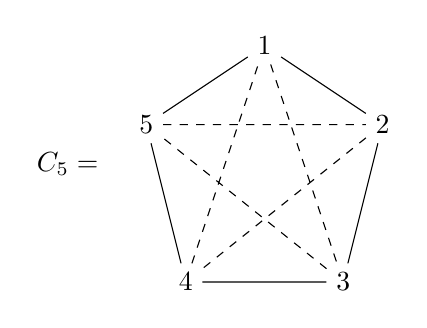
\begin{tikzpicture}
        \node(v1) at (2.5,3) {\(1\)};
        \node(v2) at (4,2) {\(2\)};
        \node(v3) at (3.5,0) {\(3\)};
        \node(v4) at (1.5,0) {\(4\)};
        \node(v5) at (1,2) {\(5\)};

        \filldraw[black] (0,1.5) circle (0pt) node[anchor=center]{\(C_5 = \)};

        \draw (v1) -- (v2) -- (v3) -- (v4) -- (v5) -- (v1);
        \draw[dashed] (v1) -- (v3) -- (v5) -- (v2) -- (v4) -- (v1);
      \end{tikzpicture}
    \end{minipage}

    We proved in Homework 1 that a self-complementary graph must have \(n = \nu \equiv 0,1 \pmod 4\).
    \begin{enumerate}
      \item (10 points) Prove that for any \(n\) divisible by 4, there exists a self-complementary graph with \(n\) vertices. \\
        (Hint: break the vertex set into 4 equal size groups and then use the path \(P_3\) as a guideline for how to connect between groups.)
        \begin{proof}
          We proceed inductively.  The base case is already outlined above as \(P_3\), so the \(n = 4\) case is a given.

          Now suppose there exists a self-complementary graph \(G\) with \(k\) vertices (\(k \equiv 0 \pmod 4\)), we show that we can use \(G\) and our path \(P_3\) to construct a self-complementary graph \(H\) with \(k + 4\) vertices.  Denote our path \(P_3\) by the sequence of vertices \(v_1-v_2-v_3-v_4\).

          To construct our new self-complementary graph \(H\), simply link every vertex in \(G\) to internal vertices \(v_2\) and \(v_3\) in \(P_3\).

          Now when we take the complement, we get the same self-complementary graph \(\overline{G}\).  All \(\overline{G}\)'s vertices link to \(v_1\) and \(v_4\) in \(\overline{P_3}\).  Since \(v_1,v_4\) are internal vertices of our new path, and \(v_2,v_3\) were internal vertices of our original path, we have that \(H\) is isomorphic to \(\overline{H}\).

          \begin{minipage}{0.4\textwidth}
            \centering
            \begin{tikzpicture}
              \node(v1) at (2,3) {\(1\)};
              \node(v2) at (2,2) {\(2\)};
              \node(v3) at (2,1) {\(3\)};
              \node(v4) at (2,0) {\(4\)};

              \filldraw[black] (0,1.5) circle (0pt) node(x)[anchor=center]{\(H :=\)};
              \filldraw[black] (1,1.5) circle (0pt) node(x)[anchor=center]{\(G\)};

              \draw (v1) -- (v2) -- (v3) -- (v4);
              \draw (x) -- (v2);
              \draw (x) -- (v3);
            \end{tikzpicture}
          \end{minipage} \(\cong\)
          \begin{minipage}{0.4\textwidth}
            \centering
            \begin{tikzpicture}
              \node(v1) at (2,3) {\(3\)};
              \node(v2) at (2,2) {\(1\)};
              \node(v3) at (2,1) {\(4\)};
              \node(v4) at (2,0) {\(2\)};

              \filldraw[black] (0,1.5) circle (0pt) node(x)[anchor=center]{\(\overline{H} :=\)};
              \filldraw[black] (1,1.5) circle (0pt) node(x)[anchor=center]{\(\overline{G}\)};

              \draw (v1) -- (v2) -- (v3) -- (v4);
              \draw (x) -- (v2);
              \draw (x) -- (v3);
            \end{tikzpicture}
          \end{minipage}

          Therefore, by the principle of induction, for any \(n\) divisible by 4, we can conclude there exists a self-complementary graph with \(n\) vertices.
        \end{proof} \n
        

      \item (10 points) Prove that for any \(n \equiv 1 \pmod 4\), there exists a self-complementary graph having \(n\) vertices. \\
        (Hint: Figure out how to add one more vertex to your construction from part (b).)
        \begin{proof}
          The same process outlined above actually applies directly to the \(n \equiv 1 \pmod 4\) case as well, with the only difference being the base case.  The base case for this being \(n=1\), and since a simple graph with one vertex can't have any edges, neither can it's complement, meaning the only possible 1-vertex simple graph is self complementary.

          With the inductive step being exactly the same, we can conclude that for any \(n \equiv 1 \pmod 1\), there exists a self-complementary graph with \(n\) edges.
        \end{proof}
        
    \end{enumerate}

    \item (20 points) Let \(G = (V,E)\) be a simple graph with \(d_G(v) \geq 2\) for all vertices \(v \in V\).  Prove that there exists a \textbf{connected} simple graph \(H\) having the same (weakly decreasing reordered) degree sequence \(\textbf{d}(H) = (d_1, \hdots, d_n) = \textbf{d}(G)\) as the one for \(G\).
      \begin{proof}
        If \(G\) is connected then we're done (\(G = H\)), so assume \(G\) disconnected.

        Let \(V_1, \hdots, V_{\omega}\) be nonempty partitions of \(V(G)\) such that any vertices \(u,v\) are connected if and only if they belong to the same partition.  This gives us connected components \(G[V_1], \hdots, G[V_{\omega}]\) of \(G\).

        For any components \(G[V_i]\) and \(G[V_j]\), take vertices \(u_i \in V_i\) and \(u_j \in V_j\).  Since \(G\) is simple, the degree of every vertex is \(\geq 2\), and vertices are only connected to vertices in their same component, we know there exists 2 distinct vertices in \(V_i\) and two distinct vertices in \(V_j\) connected to \(u_i\) and \(u_j\) respectively.

        Choose \(v_i \in V_i\) and \(v_j \in V_j\) such that \(v_i\) adjacent to \(u_i\) and \(v_j\) adjacent to \(u_j\).  Also let \(w_i\) and \(w_j\) be the other guarunteed vertices adjacent to \(u_i\) and \(u_j\).

        Now, we can construct a new graph \(G'\) with components \(G[V_i]\) and \(G[V_j]\) merged into one (without changing degrees).  To do this, simply remove links \(u_iv_i\) and \(u_jv_j\), and add linkes \(u_iu_j\) and \(v_iv_j\).  Since links \(u_iw_i\) and \(u_jw_j\) still exist, we know that all our vertices are still connected to the other vertices in their respective components, but we also have 2 new connections between components \(G[V_i]\) and \(G[V_j]\).  So now we have one big component \(G[V_{ij}]\), and since we added and removed one edge for each vertex, the degree sequence of \(G'\) matches that of \(G\).

        Finally, we can simply repeat this process \(\omega-1\) times, with our last iteration yielding graph \(H = G^{(\omega-1)}\) with only one component (itself).

        Since this construction yields a connected graph with the same degree sequence as \(G\), we can conclude such a graph exists.
      \end{proof}
      
  \end{enumerate}
\end{document}
